This section details our experimental methodology and the  video  data sets used. We evaluate our approach on the two popular data sets
UCF-11 and Hollywood2. On both data sets, we show that our work exceeds the current state-of-the-art
results. We also vary the contribution of static and motion features for the calculation
of combined vector series and explore what is optimum contribution from each domain. We show that optimum contribution
may vary depending on the data set. We also show that static and motion features
are complementary, and provide vital information about the actions occurring in a video. We compare our three fusion models and show that
all the methods are better or on par with existing state-of-the-art. Furthermore, we highlight the importance of considering the time evolution
of sub activities in order to identify complex events by comparing the results of LSTM and Random Forest Classification algorithm(which does not capture
the temporal dynamics), when applied on our features.

\subsection{Data Sets}
\noindent
\textbf{Holywood 2} \cite{marszalek2009actions}: This consists of 12 classes of human actions distributed over 1500 video clips:
\textit{answer phone, drive car, eat, fight person, get out car, hand shake,
hug person, kiss, run, sit down, sit up, }and \textit{stand up}.
The data set is composed of video clips from 69 movies and provides a challenging task, in automatic action detection.

\noindent
\textbf{UCF-11} \cite{liu2009recognizing}: This consists over 1000
sports and home videos from YouTube. This data set contains 11 action classes:
\textit{basketball shooting, cycle, dive, golf swing, horse
back ride, soccer juggle, swing, tennis swing, trampoline
jump, volleyball spike}, and \textit{walk with a dog}. Each of the action
sets is subdivided into 25 groups sharing similar environment conditions.
This is a challenging data set with
camera jitter, cluttered backgrounds and variable illumination.


\subsection{Contribution of Static and Motion Domains}

The derivation done in Cholesky based method for fusing the static and motion vectors,
provides us an insightful intuition: we can control the contribution
of motion and static domains to the fusion vector by varying the $\rho$ value.
The derivation of $\rho$ values for different contribution ratios is illustrated in
table \ref{tbl:rho change}




\begin{table}
\caption{Derivation of $\rho$ values for different contribution levels of static and motion domains to the fused vector}\label{ta:table1}
\begin{center}
  \begin{tabular}{ | l | c | r | }
    \hline
    \textbf{Contribution to $Z$} & \textbf{$\rho$ value} & \textbf{Fusion vector} \\ \hline
    {\makecell{ 80\% Motion, 20\% Static \\ $\rho_{1}=4\rho_{2}$ }} & \makecell{$\frac{1}{4}\rho_{1}=\sqrt{1-\rho_{1}^2}$ \\ $\rho_{1} = \frac{4}{\sqrt{17}}$} & $Z=\frac{4}{\sqrt{17}}M + \frac{1}{\sqrt{17}}S$ \\ \hline
    {\makecell{ 60\% Motion, 40\% Static \\ $2\rho_{1}=3\rho_{2}$ }} & \makecell{$\frac{2}{3}\rho_{1}=\sqrt{1-\rho_{1}^2}$ \\ $\rho_{1} = \frac{3}{\sqrt{13}}$} & $Z=\frac{3}{\sqrt{13}}M + \frac{2}{\sqrt{13}}S$ \\ \hline
      {\makecell{ 50\% Motion, 50\% Static \\ $\rho_{1}=\rho_{2}$ }} & \makecell{$\rho_{1}=\sqrt{1-\rho_{1}^2}$ \\ $\rho_{1} = \frac{1}{\sqrt{2}}$} & $Z=\frac{1}{\sqrt{2}}M + \frac{1}{\sqrt{2}}S$ \\ \hline
    {\makecell{ 40\% Motion, 60\% Static \\ $3\rho_{1}=2\rho_{2}$ }} & \makecell{$\frac{3}{2}\rho_{1}=\sqrt{1-\rho_{1}^2}$ \\ $\rho_{1} = \frac{2}{\sqrt{13}}$} & $Z=\frac{2}{\sqrt{13}}M + \frac{3}{\sqrt{13}}S$ \\ \hline
     {\makecell{ 80\% Motion, 20\% Static \\ $4\rho_{1}=\rho_{2}$ }} & \makecell{$4\rho_{1}=\sqrt{1-\rho_{1}^2}$ \\ $\rho_{1} = \frac{1}{\sqrt{17}}$} & $Z=\frac{1}{\sqrt{17}}M + \frac{4}{\sqrt{17}}S$ \\ \hline
      \label{tbl:rho change}
  \end{tabular}
\end{center}

\end{table}

Results for these different contribution values for UCF-11 and Hollywood2 data sets, are shown in table \ref{tbl:rho ucf}
 and table \ref{tbl:rho hollywood2}.
We use accuracy and mean average precision as performance metrics, for UCF-11 and
Hollywood2, respectively. For UCF-11, we obtain the optimum contribution ratio as 80:20 between static and motion vectors.
For Hollywood2, it is 60:40.

\begin{table*}[]
\centering
\caption{Per-class accuracy for different contribution of static and motion vectors for UCF-11. The vectors are fused using Cholesky method. Ratios are indicated in the
format static:motion. Highest accuracy for UCF-11 is achieved using a
80:20 ratio between static and motion vectors.}\label{tbl:rho ucf}
\begin{tabular}{|l||l|l|l|l|l|l|l|}
\hline
Class           & 100:0  & 80:20     & 60:40   & 50:50    & 40:60     & 20:80   & 0:100 \\ \hline  \hline
B\_shooting      & 92.4\% & \textbf{96.3\%}   & 92.7\%  &  96.3\%  &  91.3\%   & 91.9\%  & 91.3\%  \\
Biking          & 94.3\% &  \textbf{97.8\%}   & 95.6\%  &  95.4\%  &  95.4\%   & 92.6\%  & 89.5\%   \\
Diving          & 90.3\% &  \textbf{95.8\%}   & 94.3\%  &  94.3\%  &  93.1\%   &  89.6\% & 86.2\%  \\
G\_swinging      & 93.2\% & \textbf{96.7\%}   &  96.0\% &  95.8\%  &  93.3\%   &  92.8\% & 90.5\% \\
H\_riding        & 94.0\% &  \textbf{98.0\%}   &  96.6\% &  95.6\%  &  93.1\%   &  90.2\% & 87.2\% \\
S\_juggling      & 92.4\%&  \textbf{96.5\%}    & 96.0\%  &  96.0\%  &  93.7\%   &  90.2\% & 85.4\%  \\
Swinging        & 89.3\%&  \textbf{94.3\%}    & 94.3\%  &  93.6\%  &  94.1\%   &  91.7\% & 88.2\% \\
T\_swinging      & 92.3\%& \textbf{96.9\% }    &  95.7\% &  94.5\%  &  94.1\%   &  93.3\% &  90.6\% \\
T\_jumping       & 93.7\%&  \textbf{97.6\%}    &  96.7\% &  94.5\%  &  94.1\%   &  93.1\% & 90.6\% \\
V\_spiking       & 88.2\%&  93.4\%    &  94.2\% &  \textbf{97.2\%}  &  94.1\%   &  93.0\% & 89.3\% \\
W\_dog           & 90.2\%&  \textbf{96.7\% }   &   96.2\%&  95.4\%  &  93.3\%   &  91.9\% & 87.2\% \\  \hline
Accuracy        &   91.8\%&  \textbf{96.3\%}    &   95.3\%&  95.3\%  &  93.6\%   & 91.8\%  & 88.72\%  \\ \hline
\end{tabular}
\end{table*}

\begin{table*}[]
\centering
\caption{mAP for each class for different contribution of static and motion vectors to the fused vector for Hollywood2. ratios are indicated in the
format static:motion. Highest mAP for Hollywood2 is achieved using a
80:20 ratio between static and motion vectors.}\label{tbl:rho hollywood2}
\begin{tabular}{|l||l|l|l|l|l|l|l|}
\hline
Class           & 100:0 & 80:20 & 60:40 & 50:50 & 40:60 & 20:80 & 0:100 \\ \hline \hline
AnswerPhone     & 52.3\%& \textbf{76.6\%}& 49.6\%& 42.4\%& 38.2\%& 36.6\%& 28.2\%        \\
DriveCar        & 54.6\%& \textbf{98.1\%}& 49.2\%& 42.5\%& 39.1\%& 37.7\%& 26.4\%            \\
Eat             & 50.0\%& \textbf{62.1\%}& 55.6\%& 53.2\%& 53.2\%& 50.1\%& 40.0\%           \\
FightPerson     & 72.2\%& \textbf{94.3\%}& 80.2\%& 72.8\%& 66.6\%& 57.4\%& 42.2\%  \\
GetOutCar       & 56.9\%& \textbf{77.4\%}& 56.2\%& 50.2\%& 47.3\%& 40.2\%& 35.5\%\\
HandShake       & 42.2\%& 78.9\%& \textbf{80.2\%}& 72.7\%& 64.4\%& 50.3\%& 42.7\% \\
HugPerson       & 49.9\%& \textbf{77.1\%}& 64.3\%& 62.6\%& 57.2\%& 50.9\%& 40.6\% \\
Kiss            & 49.9\%& 85.3\%& \textbf{86.4\%}& 70.2\%& 68.7\%& 60.8\%& 45.5\% \\
Run             & 60.2\%& 78.2\%& \textbf{94.8\%}& 88.2\%& 82.3\%& 72.2\%& 64.5\%  \\
SitDown         & 80.2\%& 86.2\%& \textbf{91.6\%}& 80.4\%& 76.9\%& 67.3\%& 56.9\%  \\
SitUp           & 58.7\%& 75.0\%& \textbf{78.2\%}& 70.2\%& 67.4\%& 51.8\%& 47.2\% \\
StandUp         & 55.5\%& 81.2\%& \textbf{97.4\%}& 73.6\%& 62.1\%& 48.3\%& 32.3\% \\ \hline
mAP             &       &       &       &       &       &       & \\ \hline

\end{tabular}
\end{table*}

An overview distribution of the overall performance over different contribution levels, from static and motion domains, for both data sets is shown in Fig. \ref{contribution chart}.
We can see that the performance change for different contribution percentages of motion and static domain. Also, the optimum contribution may change
depending on the nature of the data set. For example, if the motion patterns are indistinguishable across actions, static information plays
a critical role, for determining the action, and vise versa. This highlights
our hypothesis, that being able to control this contribution explicitly, is vital for an action recognition system.


\pgfplotstableread[row sep=\\,col sep=&]{
    class     &   & RF  \\
    Bshooting   & 96.3  & 90.2   \\
    Biking       & 97.8 & 93.2    \\
    Diving       & 95.8 & 93.2 \\
    Gswinging   & 96.7 & 90.3  \\
    Hriding     & 98.0  & 92.3 \\
    Sjuggling   & 96.5  & 93.8  \\
    Swinging     & 94.3  & 89.2  \\
    Tswinging   & 96.9  & 91.3  \\
    Tjumping    & 97.6  & 94.5  \\
    Vspiking    & 93.4  & 89.6  \\
    Wdog        & 96.7  & 91.9  \\
    Accuracy     & 96.3  & 84.32  \\
    }\mydata


\begin{figure}
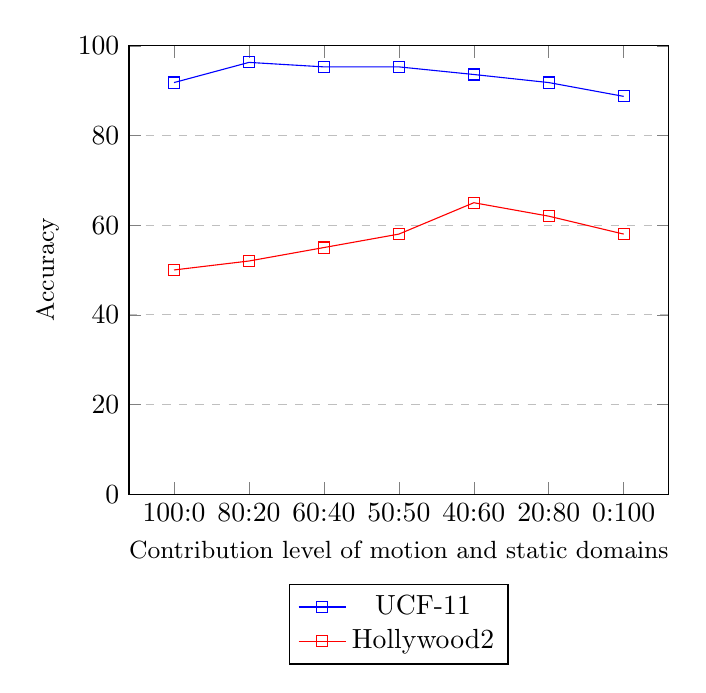
\begin{tikzpicture}
\begin{axis}[
    title={},
    xlabel={Contribution level of motion and static domains},
    ylabel={Accuracy},
    ymin=0, ymax=100,
    symbolic x coords={100:0,80:20,60:40,50:50,40:60,20:80,0:100},
    ytick={0,20,40,60,80,100,120},
    legend pos=north west,
    ymajorgrids=true,
    label style={font=\small},
    grid style=dashed,
    legend style={at={(0.5,-0.2)},anchor=north}
]

\addplot[
    color=blue,
    mark=square,
    ]
    coordinates {
    (100:0,91.8)(80:20,96.3)(60:40,95.3)(50:50,95.3)(40:60,93.6)(20:80,91.8)(0:100,88.72)
    };
    \addlegendentry{UCF-11}

    \addplot[
    color=red,
    mark=square,
    ]
    coordinates {
    (100:0,50)(80:20,52)(60:40,55)(50:50,58)(40:60,65)(20:80,62)(0:100,58)
    };
    \addlegendentry{Hollywood2}
\end{axis}
\end{tikzpicture}
\caption{Accuracy distribution for different contribution levels of motion and static domains.
This figure illustrates that motion:static ratio affects the accuracy and the optimum contribution depends on the data set.}
\label{contribution chart}
\end{figure}


\subsection{Mathematical Validation of Optimum Contribution}

As it is evident from the results of table \ref{tbl:rho ucf} and table \ref{tbl:rho hollywood2}, we experimentally obtain the
optimum contribution ratio for each data set as 80:20 and 60:40, for UCF-11 and Hollywood2, respectively. In section III, in the derivation of the variance ratio based fusion model,
we mathematically obtained values for the optimum contribution as 70:30 and 60:40 for the same data sets. It should be noted that these values closely
represent the experimental values, and hence, the results are further verified.

\subsection{Comparison of Fusion Models}
The per-class accuracies obtained for each fusion model is illustrated in table \ref{tbl:per-action fusionucf} and
table \ref{tbl:per-action fusionhollywood}. Although all three methods give impressive results, Cholesky based fusion
model is superior, and has an overall accuracy of 96.3\% for UCF-11. For Hollywood2 data set, it achieves a mean average precision
of .


\begin{table}[]
\centering
\caption{Comparison of fusion models on UCF-11 data set.}\label{tbl:per-action fusionucf}
\begin{tabular}{|l||l|l|l|l|l|}
\hline
Class            & Cholesky & Variance ratio & PCA   \\ \hline  \hline
B\_shooting       & \textbf{96.3\%}    &  90.3\%   &  90.6\%  \\
Biking           & \textbf{97.8\%}    &  90.8\%   &  91.0\%    \\
Diving           & \textbf{95.8\%}    &  92.3\%   &  89.3\%   \\
G\_swinging       & \textbf{96.7\%}    &  90.3\%   &  92.3\%   \\
H\_riding         & \textbf{98.0\%}    &  87.4\%   &  88.6\%    \\
S\_juggling       & \textbf{96.5\%}    &  89.7\%   &  92.8\%    \\
Swinging         & \textbf{94.3\%}    &  90.0\%   &  88.0\%    \\
T\_swinging       & \textbf{96.9\%}    &  89.4\%   &  93.0\%   \\
T\_jumping        & \textbf{97.6\%}    &  92.5\%   &  91.0\%    \\
V\_spiking        &\textbf{93.4\%}    &  91.6\%   &  91.7\%   \\
W\_dog            & \textbf{96.7\%}    &  91.6\%   &  93.4\%   \\ \hline \hline
Accuracy &  96.3\%   &  90.5\%   &   91.06\%   \\ \hline
\end{tabular}
\end{table}

\begin{table}[]
\centering
\caption{Comparison of fusion models on Hollywood2 data set}\label{tbl:per-action fusionhollywood}
\begin{tabular}{|l||l|l|l|l|l|}
\hline
Class            & Cholesky & Variance ratio & PCA   \\ \hline  \hline
AnswerPhone      & \textbf{76.6\%}& 62.4\%    & 67.6\%           \\
DriveCar         & \textbf{98.1\%}& 72.8\%    & 70.0\%       \\
Eat              & \textbf{62.1\%}& 49.4\%    & 56.5\%          \\
FightPerson      & \textbf{94.3\%}& 78.2\%    & 72.6\%         \\
GetOutCar        & \textbf{77.4\%}& 46.9\%    & 56.7\%          \\
HandShake        & \textbf{78.9\%}         & 56.9\%    & 55.6\%            \\
HugPerson        & \textbf{77.1\%}& 52.4.6\%    & 60.6\%            \\
Kiss             &\textbf{85.3\%}         & 64.0\%    & 66.6\%           \\
Run              & \textbf{78.2\%}         & 58.3\%    & 54.3\%            \\
SitDown          & \textbf{86.2\%}         & 72.0\%    & 68.6\%            \\
SitUp            & \textbf{75.0\%}         & 50.0\%    & 54.7\%          \\
StandUp          & \textbf{81.2\%}         & 54.4\%    & 50.0\%          \\ \hline
mAP              &                &           &                    \\ \hline
\end{tabular}
\end{table}


\subsection{Comparison with the state-of-the-art}

Table \ref{tbl:comparison} compares our results to state of the art. We use a motion:static ratio of 20:80 for UCF-11 and 60:40
for Hollywood2 to combine the static and motion vectors,
since these values gave the best results for the corresponding data sets. On UCF-11, we significantly outperform
the state of the art Ramasinghe \emph{et al.}~\cite{7486474} by 3.2\%. A mean average precision of \% is achieved by our system for Hollywood2, which outperforms
the state-of-the-art by \%.

\begin{table}[]
\centering
\caption{Comparison of our method with state-of-the-art methods in the literature. Motion:static ratios are 20:10 and 60:40 for
UCF-11 and Hollywood2 respectively.}\label{tbl:comparison}
\begin{tabular}{|l|l||l|l|}
\hline
\multicolumn{2}{|c||}{UCF-11}    & \multicolumn{2}{c|}{Hollywood2} \\ \hline
Liu \textit{et al.}\cite{liu2009recognizing}            & 71.2\%  & Vig \textit{et al.}\cite{vig2012space}           & 59.4\%      \\
Ikizler-Cinbis \textit{et al.}\cite{ikizler2010object} & 75.21\% & Jiang \textit{et al.}\cite{jiang2012trajectory}      & 59.5\%      \\
Wang \textit{et al.}\cite{wang2011action}    & 84.2\%  & Mathe \textit{et al.}\cite{mathe2012dynamic}         & 61.0\%      \\
Sameera \textit{et al.}\cite{7486474}         & 93.1\%        & Jain \textit{et al.}\cite{jain2013better}           & 62.5\%      \\
                      &         & Wang \textit{et al.}\cite{wang2011action}             & 58.3\%      \\
                      &         & Wang \textit{et al.}\cite{wang2013action}          & 64.3\%      \\ \hline \hline
Our method(Cholesky)  & \textbf{96.3\%}       & Our method        &             \\ \hline

\end{tabular}

\end{table}



\begin{table*}[]
\centering
\caption{Per-class accuracy comparison with state-of-the-art on UCF-11.}\label{tbl:per-action ucf}
\begin{tabular}{|l||l|l|l|l|l|}
\hline
Class            & Ours(Cholesky) & KLT\cite{lucas1981iterative} & Wang et al.\cite{wang2011action} & Ikizler-Cinbis\cite{ikizler2010object} & Sameera et. al.\cite{7486474} \\ \hline  \hline
B\_shooting       & \textbf{96.3\%}    &  34.0\%   &  43.0\%   & 48.5\%    &   95.6\%  \\
Biking           & \textbf{97.8\%}    &  87.6\%   &  91.7\%   & 75.17\%    &  93.1\%   \\
Diving           & 95.8\%    &  \textbf{99.0\%}   &  \textbf{99.0\%}   & 95.0\%    &   92.8\%  \\
G\_swinging       & 96.7\%    &  95.0\%   &  \textbf{97.0\%}   & 95.0\%    &   95.0\%  \\
H\_riding         & \textbf{98.0\%}    &  76.0\%   &  85.0\%   & 73.0\%    &   94.3\%  \\
S\_juggling       & \textbf{96.5\%}    &  65.0\%   &  76.0\%   & 53.0\%    &   87.8\%  \\
S\_winging         & \textbf{94.3\%}    &  86.0\%   &  88.0\%   & 66.0\%    &   92.4\%  \\
T\_swinging       & \textbf{96.9\%}    &  71.0\%   &  71.0\%   & 77.0\%    &   94.9\%  \\
T\_jumping        & \textbf{97.6\%}    &  93.0\%   &  94.0\%   & 93.0\%    &   94.0\%  \\
V\_spiking        & 93.4\%    &  \textbf{96.0\%}   &  95.0\%   & 85.0\%    &   93.2\%  \\
W\_dog            & \textbf{96.7\%}    &  76.4\%   &  87.0\%   & 66.7\%    &   91.4\%  \\ \hline \hline
Accuracy &  \textbf{96.3\%}   &  79.0\%   &  84.2\%   & 75.2\%    &   93.1\%  \\ \hline
\end{tabular}
\end{table*}

\begin{table*}[]
\centering
\caption{Per-class mAP comparison with state-of-the-art on Hollywood2.}\label{tbl:per-action hollywood}
\begin{tabular}{|l|l|l|l|l|l|}
\hline
Class            & Ours           & KLT\cite{lucas1981iterative} & Wang et al.\cite{wang2011action} & Ullah\cite{ullah2010improving}   \\ \hline \hline
AnswerPhone      & \textbf{76.6\%}& 18.3\%    & 32.6\%    & 25.9\%        \\
DriveCar         & \textbf{98.1\%}& 88.8\%    & 88.0\%    & 85.9\%     \\
Eat              & \textbf{62.1\%}& 73.4\%    & 65.2\%    & 56.4\%         \\
FightPerson      & \textbf{94.3\%}& 74.2\%    & 81.4\%    & 74.9\%         \\
GetOutCar        & \textbf{77.4\%}& 47.9\%    & 52.7\%    & 44.0\%       \\
HandShake        & 78.9\%         & 18.4\%    & 29.6\%    & 29.7\%         \\
HugPerson        & \textbf{77.1\%}& 42.6\%    & 54.2\%    & 46.1\%         \\
Kiss             & 85.3\%         & 65.0\%    & 65.8\%    & 55.0\%         \\
Run              & 78.2\%         & 76.3\%    & 82.1\%    & 69.4\%         \\
SitDown          & 86.2\%         & 59.0\%    & 62.5\%    & 58.9\%         \\
SitUp            & 75.0\%         & 27.7\%    & 20.0\%    & 18.4\%         \\
StandUp          & 81.2\%         & 63.4\%    & 65.2\%    & 57.4\%         \\ \hline
mAP              &                &           &           &          \\ \hline
\end{tabular}
\end{table*}




Per-action class results, are also compared in table \ref{tbl:per-action udf} and table \ref{tbl:per-action hollywood}. In UCF-11, our method excells
in 8 out of 11 classes, when compared with Lucas et al.\cite{lucas1981iterative}, Wang et al.\cite{wang2011action}, Ikizler et al.\cite{ikizler2010object}
and Ramasinghe \emph{et al.}~\cite{7486474}. In Hollywood2,
we calculate the average precision of each class, and compare with Lucas et al.\cite{lucas1981iterative}, Wang et al.\cite{wang2011action}, and \cite{ullah2010improving}.
We achieve best results in 10 out of 12 classes in this case.






\subsection{Effectiveness of Capturing Time Evolution}
As discussed in earlier sections, complex actions are composed of sub activities preserving
a temporal pattern. In this work, we try to capture those underlying patterns by a LSTM network.
It is interesting to verify whether this strategy has an impact on the accuracy of the
classification. Here we directly feed the fused vectors to a random forest classifier, which
does not capture sequential dynamic patterns, and compare it with the results obtained by
the LSTM network. The results are shown in Fig. \ref{randomucf} and Fig. \ref{randomHollywood}.


As it is evident from the results in in Fig. \ref{randomucf} and Fig. \ref{randomHollywood}, LSTM network significantly outperforms the
random forest classifier for both data sets. In Hollywood2, the LSTM network wins by a 12\% margin. In UCF-11, the LSTM network wins by a 12\% margin.
Therefore, it can be concluded that, exploiting
temporal patterns of sub activities, benefits complex action classification.



\pgfplotstableread[row sep=\\,col sep=&]{
    class     & LSTM & RF  \\
    B\_shooting   & 96.3  & 90.2   \\
    Biking       & 97.8 & 93.2    \\
    Diving       & 95.8 & 93.2 \\
    G\_swinging   & 96.7 & 90.3  \\
    H\_riding     & 98.0  & 92.3 \\
    S\_juggling   & 96.5  & 93.8  \\
    Swinging     & 94.3  & 89.2  \\
    T\_swinging   & 96.9  & 91.3  \\
    T\_jumping    & 97.6  & 94.5  \\
    V\_spiking    & 93.4  & 89.6  \\
    W\_dog        & 96.7  & 91.9  \\
    Accuracy     & 96.3  & 84.32  \\
    }\mydata

  \begin{figure}
   \begin{tikzpicture}
    \begin{axis}[
            ybar,
            bar width=.1cm,
            width=0.5\textwidth,
            height=.2\textwidth,
            legend pos=north west,
            label style={font=\small},
    ymajorgrids=true,
    grid style=dashed,
    legend style={at={(0.5,-0.5)},anchor=north},
            symbolic x coords={B\_shooting,Biking,Diving,G\_swinging,H\_riding,S\_juggling,Swinging,T\_swinging,T\_jumping,V\_spiking,W\_dog,Accuracy},
            x tick label style={rotate=45, anchor=north east, inner sep=0mm},
            xtick=data,
            ymin=0,ymax=100,
            xlabel={Action Classes},
            ylabel={Accuracy},
        ]
        \addplot table[x=class,y=LSTM]{\mydata};
        \addplot table[x=class,y=RF]{\mydata};
        \legend{LSTM, Random Forest}
    \end{axis}
\end{tikzpicture}
\caption{Accuracy comparison between Random Forest Classifier and LSTM for UCF-11 data set. Motion:static ratio of 20:80 is used. Accuracy is significantly higher
when the temporal dynamics of sub events are captured.}
\label{randomucf}
\end{figure}

\pgfplotstableread[row sep=\\,col sep=&]{
class     & LSTM & RF  \\
AnswerPhone      & 76.6    & 70.2    \\
DriveCar         & 98.1   & 90.4   \\
Eat              & 62.1 & 58.4       \\
FightPerson      & 94.3 &  90.0    \\
GetOutCar        & 77.4  & 60.2  \\
HandShake        & 78.9          & 74.2     \\
HugPerson        & 77.1   & 42.6      \\
Kiss             & 85.3          & 82.3     \\
Run              & 78.2          & 70.3     \\
SitDown          & 86.2          & 80.4     \\
SitUp            & 75.0          & 71.2      \\
StandUp          & 81.2          & 76.6      \\ 
mAP              &                &                   \\
    }\mydata
    
    

  \begin{figure}
   \begin{tikzpicture}
    \begin{axis}[
            ybar,
            bar width=.1cm,
            width=0.5\textwidth,
            height=.2\textwidth,
            legend pos=north west,
            label style={font=\small},
    ymajorgrids=true,
    grid style=dashed,
    legend style={at={(0.5,-0.5)},anchor=north},
            symbolic x coords={AnswerPhone,DriveCar,Eat,FightPerson,GetOutCar,HandShake,HugPerson,Kiss,Run,SitDown,SitUp,StandUp,mAP},
            x tick label style={rotate=45, anchor=north east, inner sep=0mm},
            xtick=data,
            ymin=0,ymax=100,
            xlabel={Action Classes},
            ylabel={Accuracy},
        ]
        \addplot table[x=class,y=LSTM]{\mydata};
        \addplot table[x=class,y=RF]{\mydata};
        \legend{LSTM, Random Forest}
    \end{axis}
\end{tikzpicture}
\caption{mAP comparison for Random Forest Classifier and LSTM for Hollywood2 data set. Motion:static ratio of 20:80 is used. mAP is significantly higher
when the temporal dynamics of sub events are captured.}
\label{randomHollywood}
\end{figure}

